%% CMPB submission draft converted from the MICCAI 2026 manuscript.
%% Compile from this directory with:
%%   pdflatex main
%%   bibtex main
%%   pdflatex main
%%   pdflatex main

% tectonic main.tex
% Use final,5p,times,twocolumn for the journal-style layout.
\documentclass[preprint,12pt]{elsarticle}

\usepackage{amsmath}
\usepackage{amssymb}
\usepackage{booktabs}
\usepackage{multirow}
\usepackage[table]{xcolor}
\usepackage{graphicx}
\usepackage{placeins}
\usepackage[hyphens]{url}

\biboptions{numbers,sort&compress}

\journal{Computer Methods and Programs in Biomedicine}

\begin{document}

\begin{frontmatter}

\title{Bridging weak supervision and promptable segmentation: Adapting SAM3 for medical imaging with sparse scribbles}

%% Replace placeholders before submission. CMPB uses single-anonymized review,
%% so the final submission normally includes author names and affiliations.
\author[inst1,inst2]{Qi Gao}
\author[inst1,inst2]{Huihui Fang\corref{cor1}}
\ead{hhfang@ieee.org}
\author[inst1,inst2]{Yanwu Xu}

\cortext[cor1]{Corresponding author.}

\affiliation[inst1]{
  organization={School of Future Technology, South China University of Technology},
  city={Guangzhou},
  country={China}
}

\affiliation[inst2]{
  organization={Pazhou Lab},
  city={Guangzhou},
  country={China}
}

\begin{abstract}
Text-prompted foundation models, such as Segment Anything Model 3 (SAM3), provide a flexible segmentation interface, but adapting them to medical imaging commonly requires expensive dense pixel-level annotations. Sparse scribbles offer a more economical supervision signal, yet they are incompatible with the dense masks and geometric targets assumed by the standard SAM3 training objective. We propose SAM3-Scribble, a scribble-supervised adaptation of SAM3 for text-prompted medical image segmentation. The method combines hybrid Low-Rank Adaptation (LoRA), which reduces the number of trainable parameters from approximately 840M to 11.1M, with an objective reformulation for sparse labels. Specifically, we introduce partial mask losses that restrict mask gradients to explicitly labeled pixels, and remove bounding-box regression losses and geometric matching costs that cannot be reliably derived from scribbles. Experiments on ACDC, BTCV\_cervix, and PROMISE12 show that SAM3-Scribble achieves an average Dice similarity coefficient (DSC) of 86.27\%. It improves over the strongest static scribble-supervised baseline in DSC on all three datasets and remains close to the fully supervised SAM3 counterpart. These results indicate that promptable segmentation foundation models can be adapted to multiple medical segmentation tasks under substantially reduced annotation requirements.
\end{abstract}

\begin{highlights}
\item SAM3-Scribble adapts SAM3 to medical segmentation from sparse scribbles.
\item Sparse labels are handled by partial losses and geometry-free matching.
\item Hybrid LoRA adapts the text-image pathway with 11.1M trainable parameters.
\item SAM3-Scribble outperforms static scribble baselines on three datasets.
\item The model reaches 86.27\% average DSC and approaches SAM3-Full.
\end{highlights}

\begin{keyword}
Medical image segmentation \sep Weak supervision \sep Scribble annotation \sep SAM3 \sep Foundation models \sep Low-rank adaptation
\end{keyword}

\end{frontmatter}

\section{Introduction}

Accurate medical image segmentation is a fundamental step in many computer-aided diagnosis, treatment planning, and quantitative image analysis workflows. Deep segmentation networks, from U-Net~\cite{ronneberger2015unet} to nnU-Net~\cite{isensee2021nnunet}, have achieved strong performance when sufficient pixel-level annotations are available. In clinical datasets, however, dense masks are expensive to obtain because they require experts to delineate complete anatomical boundaries slice by slice. This annotation burden becomes especially limiting when segmentation models must be adapted across organs, modalities, and institutions.

Promptable foundation models offer a complementary direction. The Segment Anything Model (SAM)~\cite{kirillov2023sam} and its successors such as SAM3~\cite{carion2025sam3} support segmentation conditioned on user prompts rather than a fixed task-specific output head. Recent biomedical foundation models, including BiomedParse~\cite{zhao2025biomedparse}, SAT~\cite{zhao2025sat}, and VoxTell~\cite{rokuss2026voxtell}, further suggest that semantic or free-text prompts can provide a flexible interface for specifying anatomical targets. Nevertheless, adapting these models to medical images still commonly relies on dense masks or large fully annotated datasets, leaving the annotation bottleneck largely unresolved.

\begin{figure}[t]
\centering
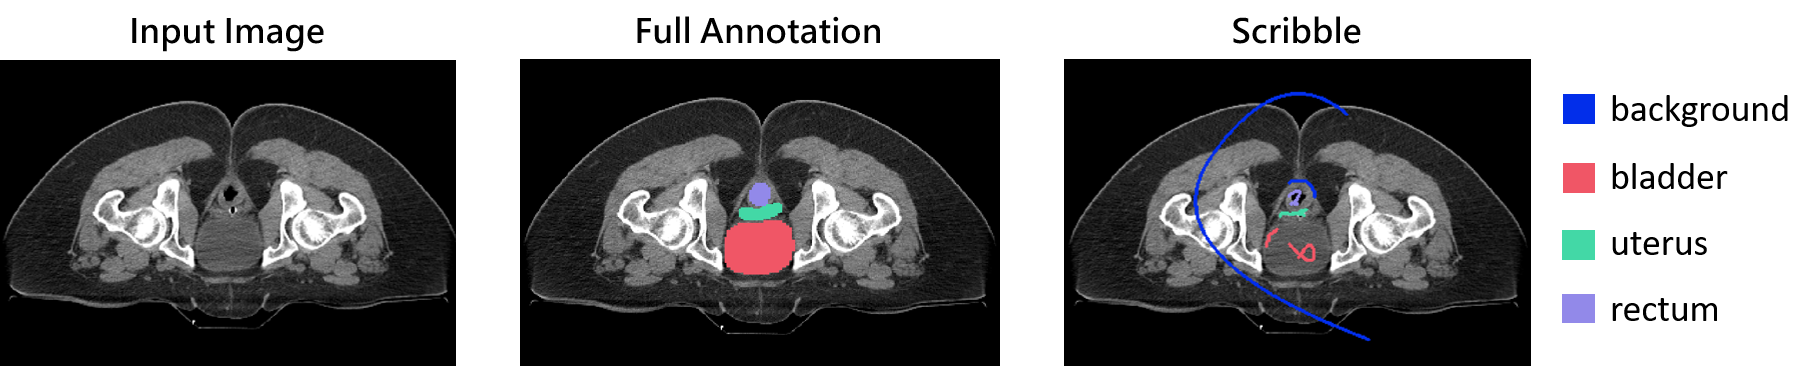
\includegraphics[width=\textwidth]{scribble.png}
\caption{Comparison between dense pixel-level annotations and sparse scribble annotations on the BTCV\_cervix dataset. Full annotation requires precise boundary contouring, whereas scribble supervision uses minimal interior hints for the target organs (bladder, uterus, and rectum) and sparse background scribbles.}
\label{fig:annotation_comparison}
\end{figure}

Scribble annotations provide a practical compromise between dense masks and image-level labels. As shown in Fig.~\ref{fig:annotation_comparison}, sparse scribbles can identify target and background regions with substantially less effort than exhaustive boundary tracing, while retaining spatial information that is absent from classification labels. Scribble-supervised medical segmentation has therefore attracted increasing attention~\cite{han2024DMSPS,li2024ScribFormer,liu2025effdnet}. These methods demonstrate that useful segmentation models can be trained from sparse labels, but they are mostly designed for static CNN or Transformer segmentation architectures. Benchmarks such as ScribbleBench~\cite{gotkowski2025scribblebench} also indicate that task-specific scribble modules do not always generalize consistently across heterogeneous medical targets.

Directly transferring scribble supervision to SAM3 is non-trivial. SAM3 adopts a DEtection TRansformer (DETR)-style architecture~\cite{carion2020detr,hatamizadeh2022unetr}, in which object queries are matched to target annotations through bipartite assignment. Its standard objective assumes dense masks and reliable geometric targets, including bounding boxes and Generalized IoU (GIoU)~\cite{rezatofighi2019giou}. Sparse scribbles violate these assumptions. They mark only a small subset of foreground and background pixels, leave most pixels unlabeled, and do not define faithful object extents or continuous boundaries. Treating unlabeled pixels as background would introduce false supervision, whereas deriving boxes from scribbles would provide noisy geometric signals for matching and regression.

This mismatch motivates a scribble-compatible adaptation of SAM3. Instead of using scribbles merely as prompts or converting them into dense pseudo-masks, we reformulate the SAM3 training objective so that sparse labels can supervise the text-prompted segmentation pathway directly. Low-Rank Adaptation (LoRA)~\cite{hu2021lora} is used for parameter-efficient fine-tuning, while the loss and matching design are modified to avoid unreliable geometric supervision and to restrict mask learning to explicitly labeled scribble regions.

The main contributions of this work are threefold:
\begin{itemize}
\item We adapt SAM3 to text-prompted medical segmentation using sparse scribble annotations rather than dense masks.
\item We design a scribble-compatible objective that removes unreliable box and GIoU regression losses, disables geometric costs in query matching, and applies partial mask losses only on valid scribble pixels.
\item We show on ACDC~\cite{bernard2018acdc}, BTCV\_cervix~\cite{landman2015btcv}, and PROMISE12~\cite{litjens2014promise} that SAM3-Scribble outperforms static scribble-supervised baselines in Dice similarity coefficient (DSC) while approaching the fully supervised SAM3 upper bound.
\end{itemize}

\section{Related work}
\label{sec:related_work}

\subsection{Promptable foundation models for medical image segmentation}

SAM introduced a promptable segmentation paradigm in which points, boxes, or masks can specify target objects without training a new task-specific head~\cite{kirillov2023sam}. This idea has rapidly motivated medical adaptations. SAMed~\cite{zhang2023samed}, Medical SAM Adapter~\cite{wu2025medicalsamadapter}, SAM-Med2D~\cite{cheng2023sammed2d}, and MedSAM~\cite{ma2024medsam} adapt SAM to medical images through fine-tuning, adapters, or large-scale medical segmentation data. Other studies extend promptable segmentation from 2D images to volumetric or temporal settings, including 3DSAM-adapter~\cite{gong2024threedsamadapter}, MA-SAM~\cite{chen2023masam}, and MedSAM2~\cite{ma2025medsam2}. In parallel, text-prompted biomedical foundation models such as BiomedParse~\cite{zhao2025biomedparse}, SAT~\cite{zhao2025sat}, and VoxTell~\cite{rokuss2026voxtell} broaden the prompt interface from spatial hints to semantic descriptions.

These methods improve the flexibility and generality of medical image segmentation, but most are trained or adapted with dense segmentation masks. Their prompts are usually treated as inference-time interaction signals or task specifications, whereas the supervision itself remains fully annotated. Our work instead focuses on adapting a text-prompted segmentation foundation model when only sparse scribble labels are available for training.

\subsection{Scribble-supervised medical image segmentation}

Scribble supervision reduces annotation cost by labeling only sparse foreground or background traces. Early weakly supervised segmentation work introduced partial losses and label propagation for learning from scribbles~\cite{lin2016ScribbleSup}, while medical studies further explored geodesic priors and interactive weak labels~\cite{wang2018deepigeos}. Recent medical scribble-supervised methods improve the use of sparse labels through pseudo-label expansion, consistency regularization, hybrid architectures, and feature-level priors. For example, CycleMix augments scribble supervision with mix-based consistency~\cite{zhang2022cyclemix}; DMSPS uses dynamically mixed soft pseudo-labels and uncertainty-guided expansion~\cite{han2024DMSPS}; ScribFormer combines CNN and Transformer branches with attention consistency~\cite{li2024ScribFormer}; and EFFDNet enhances foreground-background feature discrimination from scribble cues~\cite{liu2025effdnet}. Other recent methods address inconsistent scribble labeling with cross-image matching~\cite{chen2025crossimage}, exploit anatomy distribution priors~\cite{zhang2025medcl}, or regularize few-scribble learning across related tasks~\cite{zhang2024modelmix}.

Benchmarking studies also highlight that scribble supervision should be evaluated beyond a single cardiac dataset. Scribbles for All provides broader scribble segmentation benchmarks for natural images~\cite{boettcher2024scribblesforall}, while ScribbleBench revisits 3D medical scribble supervision across heterogeneous targets and shows that robust standardized objectives can be competitive with more specialized designs~\cite{gotkowski2025scribblebench}. ZScribbleSeg further emphasizes efficient scribble modeling and spatial or shape priors for maximizing the value of sparse labels~\cite{zhang2026zscribbleseg}. Despite these advances, most scribble-supervised medical methods are designed for static CNN or Transformer segmentation networks and do not directly address the query matching and geometric losses used by SAM3.

\subsection{Adapting segmentation foundation models with sparse supervision}

Adapting foundation models under sparse supervision differs from using sparse prompts at inference time. A point, box, or text prompt asks the model what to segment, whereas scribble supervision defines how the model should learn from incomplete labels. This distinction is important for SAM3 because its DETR-style decoder relies on bipartite query assignment~\cite{carion2020detr,kuhn1955hungarian} and geometric targets such as bounding boxes and GIoU~\cite{rezatofighi2019giou}. Dense annotations support these objectives naturally, but scribbles leave most pixels unlabeled and do not define reliable object extents.

Parameter-efficient fine-tuning methods such as LoRA~\cite{hu2021lora} make it feasible to adapt large segmentation models without updating all parameters, but they do not by themselves resolve the supervision mismatch. The central issue is objective-level compatibility: sparse scribbles should supervise only known labeled pixels, and unreliable geometric signals should not affect query assignment or regression. Our method therefore combines parameter-efficient adaptation with a reformulated SAM3 objective that removes invalid geometric losses, suppresses geometric costs in Hungarian matching, and applies partial mask supervision over valid scribble regions.

\section{Methods}
\label{sec:methods}

\subsection{SAM3 image model}

SAM3 is a promptable segmentation model composed of an image encoder, prompt encoders, and a DETR-style transformer decoder. In this study, we use the SAM3 image model and process volumetric medical images slice by slice. This design allows direct adaptation of the 2D SAM3 image model while preserving the text-prompted inference interface. The image encoder maps a 2D slice to dense visual features, the text encoder maps anatomical category names to semantic prompt embeddings, and the transformer processes learnable object queries through segmentation, score, and box heads.

For a full mask target $y_{gt}$ and query prediction $\hat{y}$, the standard SAM3 objective combines mask, box, semantic, and presence terms:
\begin{equation}
    \mathcal{L}_{SAM3} =
    \lambda_{mask}\mathcal{L}_{mask}
    + \lambda_{box}\mathcal{L}_{box}
    + \lambda_{giou}\mathcal{L}_{giou}
    + \lambda_{ce}\mathcal{L}_{ce}
    + \lambda_{presence}\mathcal{L}_{presence}.
\end{equation}
The mask loss combines focal~\cite{Lin2017focal} and Dice~\cite{milletari2016dice} losses, while $\mathcal{L}_{box}$ and $\mathcal{L}_{giou}$ enforce geometric localization~\cite{rezatofighi2019giou}. In the DETR-style decoder, SAM3 predicts a fixed set of object queries, and each ground-truth object must be assigned to one predicted query before the matched predictions can be supervised. SAM3 performs this one-to-one query assignment with a Binary Hungarian Matcher~\cite{kuhn1955hungarian} using the matching cost
\begin{equation}
    \mathcal{C}(\hat{y}_i, y_j) =
    \omega_{cls}\mathcal{C}_{cls}
    + \omega_{box}\mathcal{C}_{box}
    + \omega_{giou}\mathcal{C}_{giou}.
\end{equation}
where $\hat{y}_i$ is a query prediction and $y_j$ is a target object. The selected query-target pairs determine which predictions receive mask, semantic, presence, and geometric supervision. These geometric terms are reliable for dense annotations but problematic for sparse scribbles.

\subsection{Scribble-compatible objective}
\label{sec:scribble_objective}

\begin{figure}[t]
\centering
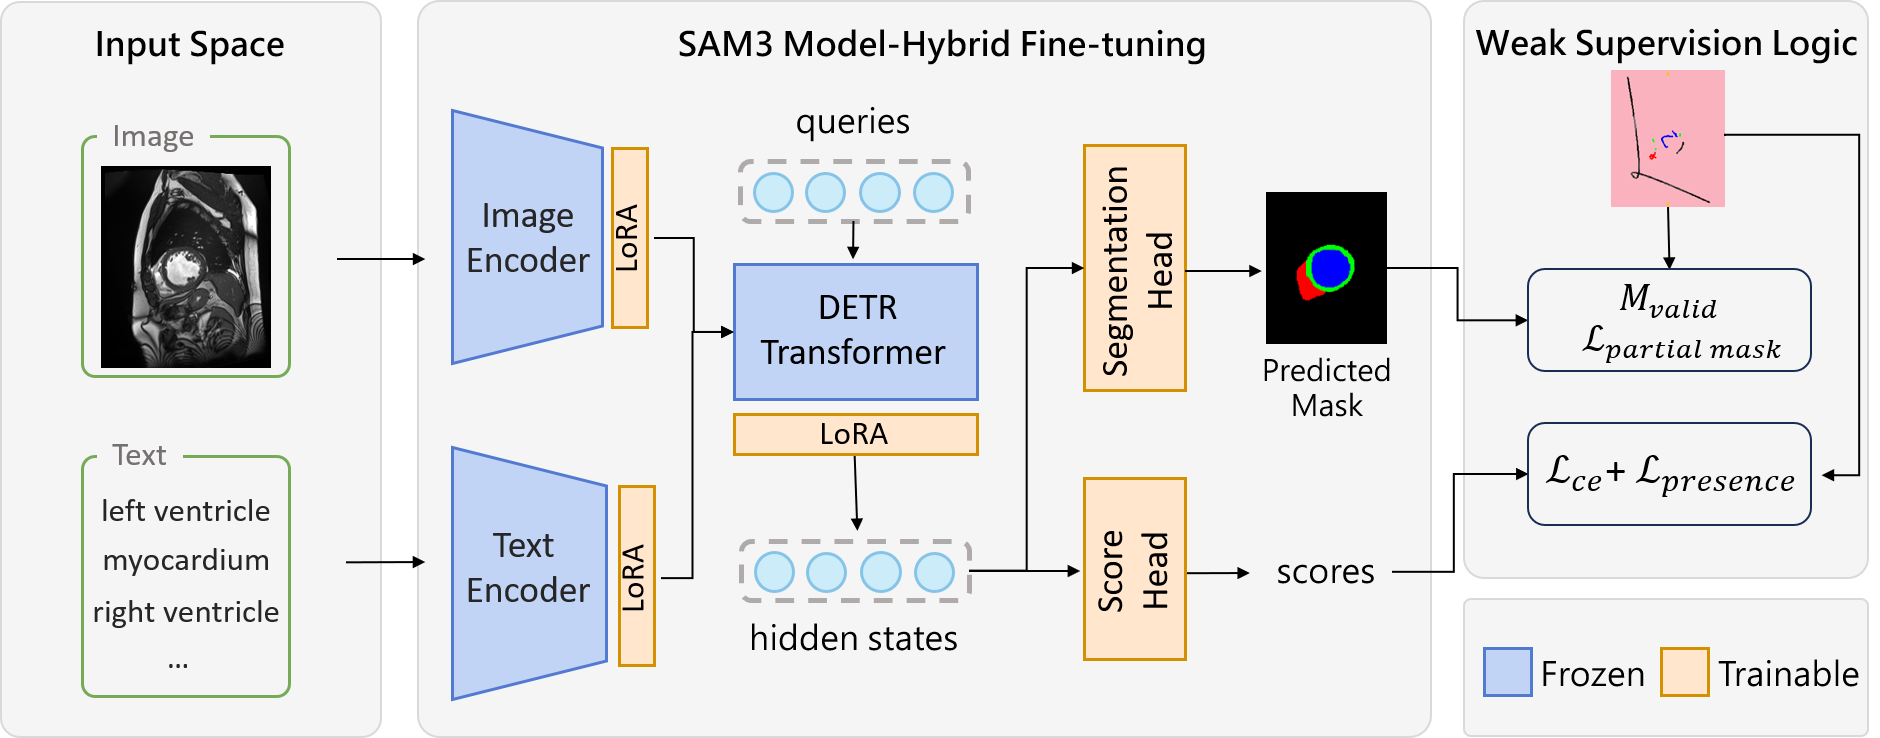
\includegraphics[width=\textwidth]{framework.png}
\caption{Overview of the proposed scribble-supervised adaptation framework. The image and text prompt are processed by SAM3 encoders and a DETR-style transformer with LoRA modules. Weak supervision is provided by a partial mask loss gated by the valid scribble region, together with semantic and presence losses derived from sparse annotations.}
\label{fig:framework}
\end{figure}

Figure~\ref{fig:framework} summarizes the adaptation framework. For each anatomical class, we construct a binary supervision target from the multi-class scribble map. Pixels marked as the queried class are assigned positive labels, pixels marked as other anatomical classes or background scribbles are assigned negative labels, and all remaining pixels are assigned the ignore label. The valid mask $M_{valid}$ is therefore the union of all annotated scribble pixels for the current slice, rather than the full image domain. This formulation uses both foreground and known-negative scribble evidence while preventing unlabeled pixels from being interpreted as background.

\subsubsection{Bypassing geometric constraints}

Scribbles provide sparse interior or boundary hints but do not define exact object extents. Consequently, bounding boxes derived from scribbles are not faithful substitutes for full-mask boxes. We therefore set the box and GIoU regression losses to zero during backpropagation:
\begin{equation}
    \lambda_{box} = \lambda_{giou} = 0.
\end{equation}
The matcher is also modified to avoid geometry-driven assignment from incomplete scribble targets. In the weakly supervised configuration, the focal classification cost is kept at $2.0$, while the box and GIoU matching costs are set from $5.0$ and $2.0$ to $0.0$ and $0.0$, respectively. This prevents scribble-derived extents from influencing Hungarian assignment.

\subsubsection{Partial mask loss}

Let $M_{valid}$ denote the binary valid-region mask and $Y_{gt}$ denote the tri-state scribble target. We define partial focal and partial Dice losses over pixels where $M_{valid}=1$ and ignore all unlabeled pixels. The total objective is
\begin{equation}
    \mathcal{L}_{total} =
    \lambda_{ce}\mathcal{L}_{ce}
    + \lambda_{presence}\mathcal{L}_{presence}
    + \lambda_{focal}\mathcal{L}_{p\_focal}
    + \lambda_{dice}\mathcal{L}_{p\_dice}.
\end{equation}
The partial focal loss is computed by applying the same valid-region mask to the pixel-wise focal loss:
\begin{equation}
    \mathcal{L}_{p\_focal} =
    \frac{\sum M_{valid} \cdot \mathcal{L}_{focal}(P, Y_{gt})}
    {\sum M_{valid} + \epsilon}.
\end{equation}
The partial Dice term is
\begin{equation}
    \mathcal{L}_{p\_dice} =
    1 -
    \frac{2\sum(P \cdot Y_{gt} \cdot M_{valid}) + \epsilon}
    {\sum(P \cdot M_{valid}) + \sum(Y_{gt} \cdot M_{valid}) + \epsilon},
\end{equation}
where $P$ is the predicted probability map. The same valid-region mask is applied to the focal term. This prevents unlabeled pixels from contributing false background gradients.

\subsection{Hybrid LoRA adaptation}

We use a hybrid parameter-efficient adaptation strategy. LoRA modules are inserted into linear layers of the image encoder, text encoder, geometry encoder, DETR encoder, DETR decoder, and mask decoder, enabling low-rank updates across the text-image segmentation pathway. In addition, the segmentation and dot-product scoring heads are fine-tuned directly because they are task-specific prediction heads. The LoRA rank is set to $8$ and the scaling parameter to $16.0$, reducing the number of trainable parameters from approximately $840$M to $11.1$M. This design preserves adaptation capacity across visual, semantic, geometric, and query-decoding components while avoiding full-model fine-tuning.

\section{Experimental setup}
\label{sec:experiments}

\subsection{Datasets and annotation protocol}

We evaluate on ACDC (MRI)~\cite{bernard2018acdc}, BTCV\_cervix (CT)~\cite{landman2015btcv}, and PROMISE12 (MRI)~\cite{litjens2014promise}. Table~\ref{tab:dataset_protocol} summarizes the patient-level splits and scribble sources. For ACDC, we use the expert scribble annotations and the train/validation/test split introduced by Valvano et al.~\cite{valvano2021scribbles}. For BTCV\_cervix, we follow the SAT evaluation split because the original BTCV challenge test labels are not publicly released. The SAT labeled set contains 30 cases, of which 24 are used as the development set and 6 as the held-out test set; we further reserve 4 cases from the 24-case development set for validation, resulting in a 20/4/6 train/validation/test split. For PROMISE12, whose released training labels do not provide a separate validation split, validation cases are sampled from the training portion and all methods are evaluated on the same held-out test cases.

ACDC therefore evaluates manually provided expert scribbles, whereas BTCV\_cervix and PROMISE12 use algorithmically generated scribbles following the ScribbleBench protocol~\cite{gotkowski2025scribblebench}, with NURBS~\cite{piegl2012nurbs} used to simulate sparse foreground traces. The foreground scribble ratio is computed on the training split as the number of foreground scribble pixels divided by the corresponding full-mask foreground pixels. Across the three datasets, scribbles cover only 5.36\%--10.91\% of the full-mask pixels, covering both expert and generated annotation regimes.

\begin{table}[!htbp]
\centering
\caption{Dataset protocol and scribble annotation statistics. Cases and images are reported as train/validation/test. Foreground scribble ratios are computed on the training split against the corresponding dense target masks.}
\label{tab:dataset_protocol}
\setlength{\tabcolsep}{3pt}
\resizebox{\textwidth}{!}{%
\begin{tabular}{l c l c c l}
\toprule
\textbf{Dataset} & \textbf{Modality} & \textbf{Targets} & \textbf{Cases} & \textbf{Images} & \textbf{Scribble source / ratio} \\
\midrule
ACDC & MRI & right ventricle, myocardium, left ventricle & 70/15/15 & 1322/314/266 & Expert~\cite{valvano2021scribbles}, 10.91\% \\
BTCV\_cervix & CT & bladder, uterus, rectum, small bowel & 20/4/6 & 3768/697/1062 & ScribbleBench-generated, 8.08\% \\
PROMISE12 & MRI & prostate & 40/10/30 & 1082/295/795 & ScribbleBench-generated, 5.36\% \\
\bottomrule
\end{tabular}
}
\end{table}

\subsection{Baselines}

We compare against text-prompted medical segmentation models, including BiomedParse-v2~\cite{zhao2025biomedparse,zhao2025boltzmann}, SAT-Pro~\cite{zhao2025sat}, and VoxTell~\cite{rokuss2026voxtell}, as well as weakly supervised static models, including ScribFormer~\cite{li2024ScribFormer}, ScribbleBench~\cite{gotkowski2025scribblebench}, and EFFDNet~\cite{liu2025effdnet}. All static scribble-supervised baselines are trained, validated, and tested with the same patient-level splits and the same scribble source as SAM3-Scribble. The text-prompted baselines are evaluated with their released pre-trained weights on the same test images, without dataset-specific fine-tuning. For these text-prompted baselines, prompts are constructed according to the text prompt conventions used in their released training or evaluation protocols, so that each model is evaluated under its recommended prompt format. Because large-scale pre-training corpora may overlap with common public medical benchmarks, methods with possible test-sample exposure are retained for context but marked as data-leakage cases in the results tables. BiomedParse-v2 and VoxTell are treated as leakage-risk cases on PROMISE12, BiomedParse-v2 and VoxTell on BTCV\_cervix, and all three text-prompted baselines on ACDC.

\subsection{Implementation details}

The model is implemented in PyTorch and initialized from the official SAM3 checkpoint. Three-dimensional volumes are processed as 2D slices. MRI preprocessing uses 0.5--99.5 percentile clipping followed by min-max normalization to $[0,255]$. CT preprocessing uses a window level of 40 HU and a window width of 400 HU before 8-bit mapping. Loss weights are set to $\lambda_{ce}=\lambda_{presence}=20$, $\lambda_{dice}=10$, and $\lambda_{focal}=200$. During inference, each anatomical target is queried using its class name as the text prompt. For multi-organ datasets, prompts are evaluated independently for each target class. The decoder generates 200 queries per slice; masks with confidence below $0.7$ are discarded, and the highest-scoring remaining mask is retained for the queried class. Slice-wise predictions are stacked to reconstruct 3D volumes. We report Dice similarity coefficient (DSC), 95th percentile Hausdorff distance (HD95), intersection over union (IoU), and normalized surface Dice (NSD), with HD95 and NSD computed using the \textit{surface-distance} library. Statistical significance is assessed using paired Wilcoxon signed-rank tests on per-case DSC scores, with Holm correction for multiple comparisons.

\section{Results}
\label{sec:results}

Tables~\ref{tab:main_results_acdc}--\ref{tab:main_results_promise12} summarize the quantitative results on the three datasets. SAM3-Scribble achieves DSC scores of 91.61\%, 76.84\%, and 90.36\% on ACDC, BTCV\_cervix, and PROMISE12, respectively, corresponding to an average DSC of 86.27\%. It consistently improves over the strongest static scribble-supervised baseline in DSC on all three datasets and remains close to the fully supervised SAM3 upper bound. On BTCV\_cervix, SAM3-Scribble slightly exceeds SAM3-Full in DSC and HD95, although both methods remain close in absolute performance.

% Generated by gq_paper/cmpb/aggregate_cmpb_results.py.

\begin{table}[!htbp]
\centering
\caption{Quantitative comparison on ACDC. Values are reported as mean $\pm$ standard deviation. Gray cells indicate data-leakage cases. Best valid scores, excluding leakage cases and the SAM3-Full upper bound, are in bold; second-best scores are underlined.}
\label{tab:main_results_acdc}
\setlength{\tabcolsep}{4pt}
\resizebox{\textwidth}{!}{%
\begin{tabular}{l c c c c c}
\toprule
\textbf{Method} & \textbf{Sup.} & \textbf{DSC (\%)} $\uparrow$ & \textbf{HD95} $\downarrow$ & \textbf{IoU (\%)} $\uparrow$ & \textbf{NSD (\%)} $\uparrow$ \\
\midrule
\textit{Text-prompted models} & & & & & \\
BiomedParse-v2 & Full & \cellcolor{gray!20}85.97 $\pm$ 10.39 & \cellcolor{gray!20}5.50 $\pm$ 5.58 & \cellcolor{gray!20}79.44 $\pm$ 10.84 & \cellcolor{gray!20}90.05 $\pm$ 10.24 \\
VoxTell & Full & \cellcolor{gray!20}87.03 $\pm$ 3.35 & \cellcolor{gray!20}1.40 $\pm$ 0.40 & \cellcolor{gray!20}77.56 $\pm$ 5.14 & \cellcolor{gray!20}98.75 $\pm$ 0.87 \\
SAT-Pro & Full & \cellcolor{gray!20}90.80 $\pm$ 1.50 & \cellcolor{gray!20}2.77 $\pm$ 0.51 & \cellcolor{gray!20}83.39 $\pm$ 2.42 & \cellcolor{gray!20}91.69 $\pm$ 2.76 \\
\midrule
\textit{Scribble-supervised static models} & & & & & \\
ScribFormer & Scrib. & 85.54 $\pm$ 5.76 & 23.74 $\pm$ 27.42 & 75.64 $\pm$ 7.74 & 86.04 $\pm$ 7.43 \\
ScribbleBench & Scrib. & 84.72 $\pm$ 10.09 & 69.45 $\pm$ 56.35 & 75.36 $\pm$ 12.13 & 84.57 $\pm$ 13.00 \\
EFFDNet & Scrib. & \underline{89.57 $\pm$ 5.06} & \underline{10.75 $\pm$ 14.09} & \underline{81.77 $\pm$ 7.03} & \underline{92.30 $\pm$ 6.45} \\
\midrule
\textit{Ours} & & & & & \\
\textbf{SAM3-Scribble} & \textbf{Scrib.} & \textbf{91.61 $\pm$ 3.64} & \textbf{3.47 $\pm$ 3.13} & \textbf{84.94 $\pm$ 5.43} & \textbf{95.42 $\pm$ 4.22} \\
SAM3-Full & Full & 92.93 $\pm$ 2.81 & 3.07 $\pm$ 2.30 & 87.09 $\pm$ 4.61 & 96.57 $\pm$ 3.08 \\
\bottomrule
\end{tabular}%
}
\end{table}

\begin{table}[!htbp]
\centering
\caption{Quantitative comparison on BTCV\_cervix. Values are reported as mean $\pm$ standard deviation. Gray cells indicate data-leakage cases. Best valid scores, excluding leakage cases and the SAM3-Full upper bound, are in bold; second-best scores are underlined.}
\label{tab:main_results_btcv}
\setlength{\tabcolsep}{4pt}
\resizebox{\textwidth}{!}{%
\begin{tabular}{l c c c c c}
\toprule
\textbf{Method} & \textbf{Sup.} & \textbf{DSC (\%)} $\uparrow$ & \textbf{HD95} $\downarrow$ & \textbf{IoU (\%)} $\uparrow$ & \textbf{NSD (\%)} $\uparrow$ \\
\midrule
\textit{Text-prompted models} & & & & & \\
BiomedParse-v2 & Full & \cellcolor{gray!20}36.43 $\pm$ 4.68 & \cellcolor{gray!20}81.60 $\pm$ 31.73 & \cellcolor{gray!20}30.38 $\pm$ 3.16 & \cellcolor{gray!20}29.39 $\pm$ 3.96 \\
VoxTell & Full & \cellcolor{gray!20}82.20 $\pm$ 2.17 & \cellcolor{gray!20}22.58 $\pm$ 6.53 & \cellcolor{gray!20}71.23 $\pm$ 3.25 & \cellcolor{gray!20}69.42 $\pm$ 5.95 \\
SAT-Pro & Full & 70.86 $\pm$ 5.39 & 33.39 $\pm$ 18.30 & 57.59 $\pm$ 6.01 & 54.99 $\pm$ 8.01 \\
\midrule
\textit{Scribble-supervised static models} & & & & & \\
ScribFormer & Scrib. & 64.14 $\pm$ 6.87 & 34.23 $\pm$ 18.86 & 50.49 $\pm$ 7.24 & 42.41 $\pm$ 8.54 \\
ScribbleBench & Scrib. & \underline{74.68 $\pm$ 2.98} & \underline{24.17 $\pm$ 9.89} & \underline{62.22 $\pm$ 3.57} & \underline{62.02 $\pm$ 7.36} \\
EFFDNet & Scrib. & 68.75 $\pm$ 9.74 & 39.88 $\pm$ 36.53 & 55.23 $\pm$ 10.63 & 51.59 $\pm$ 12.92 \\
\midrule
\textit{Ours} & & & & & \\
\textbf{SAM3-Scribble} & \textbf{Scrib.} & \textbf{76.84 $\pm$ 2.29} & \textbf{22.01 $\pm$ 6.19} & \textbf{64.51 $\pm$ 2.97} & \textbf{66.05 $\pm$ 3.66} \\
SAM3-Full & Full & 75.05 $\pm$ 2.39 & 22.34 $\pm$ 6.86 & 63.04 $\pm$ 3.09 & 66.23 $\pm$ 4.72 \\
\bottomrule
\end{tabular}%
}
\end{table}

\begin{table}[!htbp]
\centering
\caption{Quantitative comparison on PROMISE12. Values are reported as mean $\pm$ standard deviation. Gray cells indicate data-leakage cases. Best valid scores, excluding leakage cases and the SAM3-Full upper bound, are in bold; second-best scores are underlined.}
\label{tab:main_results_promise12}
\setlength{\tabcolsep}{4pt}
\resizebox{\textwidth}{!}{%
\begin{tabular}{l c c c c c}
\toprule
\textbf{Method} & \textbf{Sup.} & \textbf{DSC (\%)} $\uparrow$ & \textbf{HD95} $\downarrow$ & \textbf{IoU (\%)} $\uparrow$ & \textbf{NSD (\%)} $\uparrow$ \\
\midrule
\textit{Text-prompted models} & & & & & \\
BiomedParse-v2 & Full & \cellcolor{gray!20}85.97 $\pm$ 6.31 & \cellcolor{gray!20}14.78 $\pm$ 13.63 & \cellcolor{gray!20}75.90 $\pm$ 9.29 & \cellcolor{gray!20}76.01 $\pm$ 11.93 \\
VoxTell & Full & \cellcolor{gray!20}80.81 $\pm$ 13.97 & \cellcolor{gray!20}27.61 $\pm$ 31.18 & \cellcolor{gray!20}69.87 $\pm$ 17.73 & \cellcolor{gray!20}71.06 $\pm$ 18.87 \\
SAT-Pro & Full & 88.02 $\pm$ 3.73 & \textbf{4.15 $\pm$ 1.21} & 78.79 $\pm$ 5.80 & 79.82 $\pm$ 8.53 \\
\midrule
\textit{Scribble-supervised static models} & & & & & \\
ScribFormer & Scrib. & 78.13 $\pm$ 8.06 & 12.91 $\pm$ 9.14 & 64.78 $\pm$ 10.51 & 59.78 $\pm$ 13.46 \\
ScribbleBench & Scrib. & \underline{88.90 $\pm$ 2.90} & \underline{4.79 $\pm$ 1.78} & \underline{80.14 $\pm$ 4.62} & \underline{82.01 $\pm$ 5.92} \\
EFFDNet & Scrib. & 87.69 $\pm$ 3.71 & 10.67 $\pm$ 17.39 & 78.27 $\pm$ 5.74 & 79.19 $\pm$ 8.20 \\
\midrule
\textit{Ours} & & & & & \\
\textbf{SAM3-Scribble} & \textbf{Scrib.} & \textbf{90.36 $\pm$ 3.45} & 5.95 $\pm$ 6.22 & \textbf{82.58 $\pm$ 5.56} & \textbf{84.99 $\pm$ 7.29} \\
SAM3-Full & Full & 91.53 $\pm$ 2.98 & 6.05 $\pm$ 6.76 & 84.52 $\pm$ 4.95 & 87.39 $\pm$ 7.38 \\
\bottomrule
\end{tabular}%
}
\end{table}

\FloatBarrier

We performed paired Wilcoxon signed-rank tests on per-case DSC scores, with Holm correction across the reported DSC comparisons. SAM3-Scribble significantly outperforms the static scribble-supervised baselines on ACDC and PROMISE12. On BTCV\_cervix, the DSC differences are positive but do not remain significant after correction, reflecting the small test set size of six cases. The DSC gap between SAM3-Scribble and SAM3-Full is small in absolute value, but SAM3-Full remains significantly higher on ACDC and PROMISE12. Detailed p-values are provided in Supplementary Table~S9. Figure~\ref{fig:per_case_dsc_distribution} visualizes the corresponding per-case DSC distributions.

\begin{figure}[!htbp]
\centering
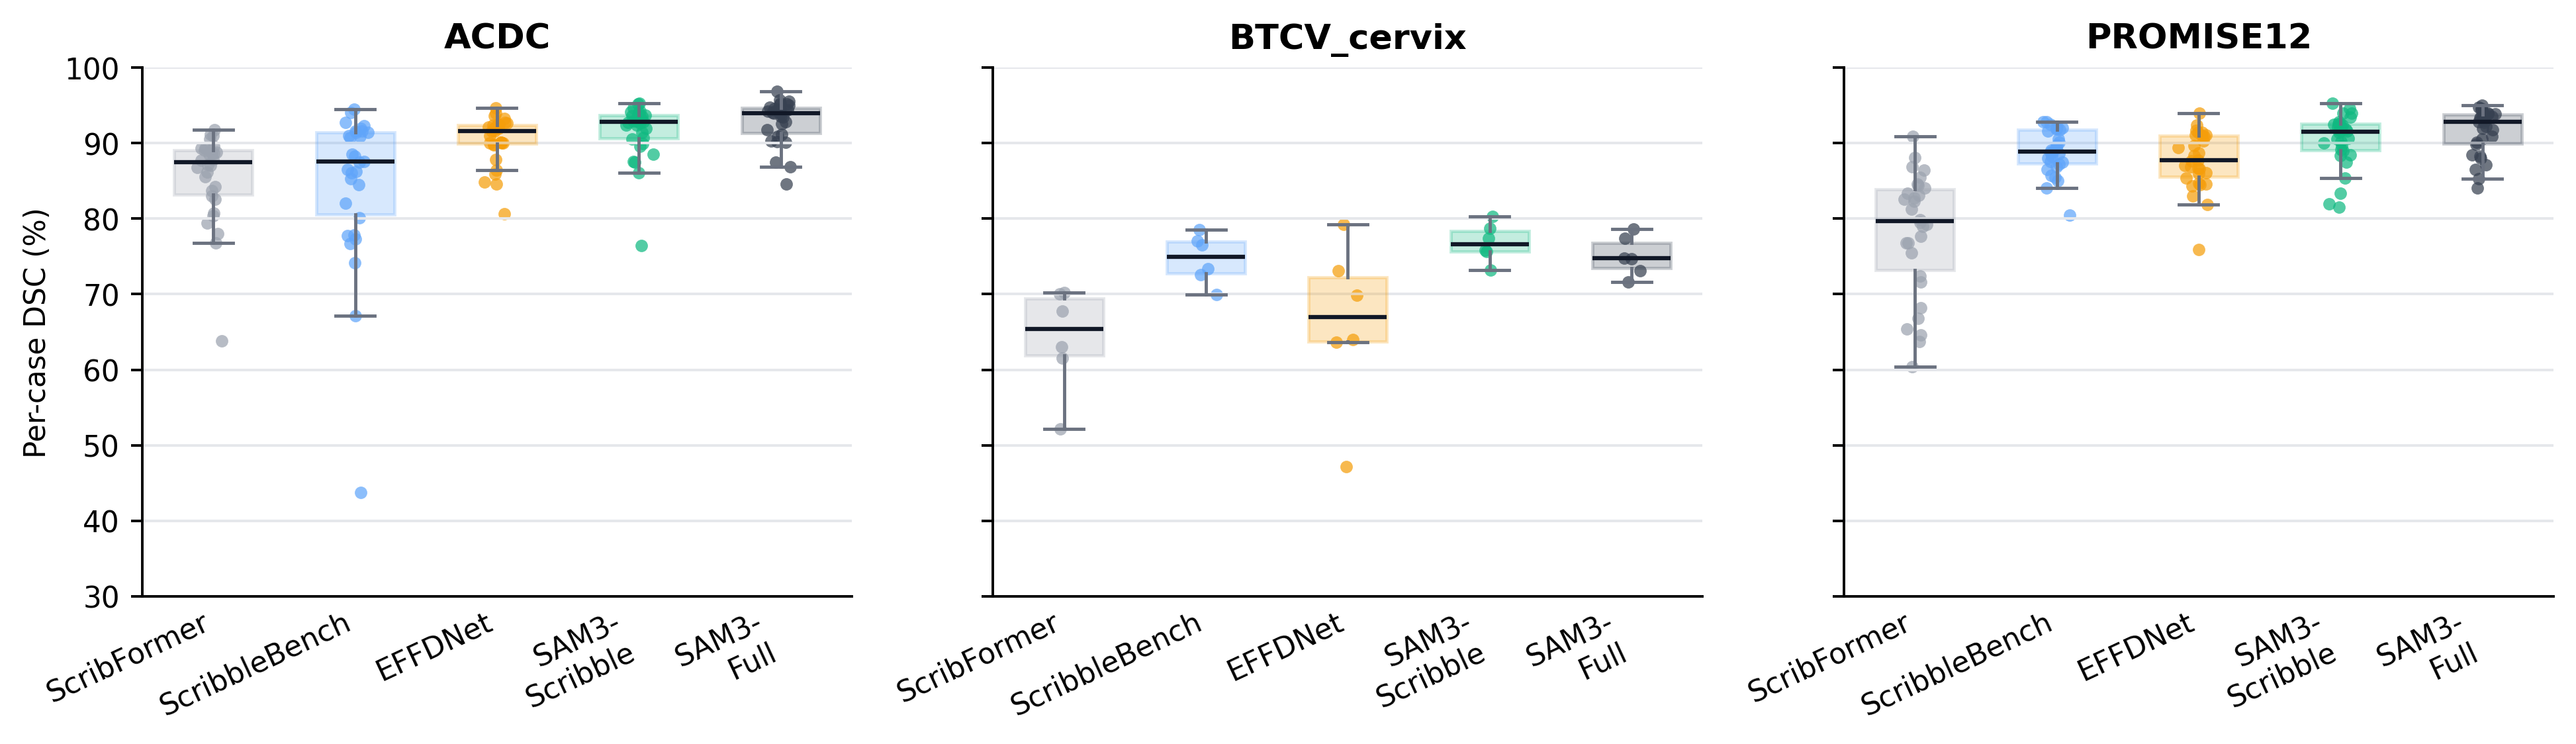
\includegraphics[width=\textwidth]{per_case_dsc_distribution.png}
\caption{Per-case DSC distributions on ACDC, BTCV\_cervix, and PROMISE12. Each point corresponds to one test case, and boxes summarize the interquartile range. SAM3-Scribble shows higher and more stable DSC distributions than the static scribble-supervised baselines on ACDC and PROMISE12, while BTCV\_cervix shows positive but less statistically stable differences due to its smaller test set.}
\label{fig:per_case_dsc_distribution}
\end{figure}

\FloatBarrier

\subsection{Ablation on scribble-compatible objectives}
\label{sec:objective_ablation}

We further examined the two geometric components that are affected by sparse scribble supervision: box/GIoU regression losses and geometric costs in Hungarian query matching. All variants use the same joint training data, partial mask loss, LoRA configuration, validation-based checkpoint selection, and test threshold unless otherwise specified.

\begin{table}[!htbp]
\centering
\caption{Ablation study of box and GIoU regression losses under scribble supervision. The matcher uses the final no-geometric setting for all variants. DSC, IoU, and NSD are macro-averaged over ACDC, BTCV\_cervix, and PROMISE12 and reported as percentages; HD95 is reported in millimeters.}
\label{tab:regression_ablation}
\setlength{\tabcolsep}{5pt}
\resizebox{\textwidth}{!}{%
\begin{tabular}{l c c c c c}
\toprule
\textbf{Variant} & \textbf{box/GIoU loss} & \textbf{DSC (\%)} $\uparrow$ & \textbf{HD95} $\downarrow$ & \textbf{IoU (\%)} $\uparrow$ & \textbf{NSD (\%)} $\uparrow$ \\
\midrule
\textbf{No geometric regression (ours)} & \textbf{0/0} & \textbf{86.27} & 10.48 & \textbf{77.35} & \textbf{82.15} \\
Full geometric regression & 5/2 & 85.86 & \textbf{10.27} & 76.75 & 81.65 \\
Reduced geometric regression & 1/1 & 85.95 & 11.32 & 76.99 & 81.87 \\
\bottomrule
\end{tabular}%
}
\end{table}

Table~\ref{tab:regression_ablation} shows that removing scribble-derived box and GIoU regression losses gives the best overall DSC and NSD. Restoring the original geometric regression loss slightly improves HD95 but lowers overlap and surface Dice metrics, while a reduced geometric loss remains below the proposed setting. These results support removing geometric regression as an unreliable supervision target when object extents are inferred only from sparse scribbles.

We also examined whether geometric costs should be retained in Hungarian query assignment under scribble supervision. Since scribbles do not define faithful object extents, bounding boxes derived from sparse annotations may introduce noisy assignment signals. We therefore compared the original SAM3 matcher, two reduced-geometry variants, and the final no-geometric matcher while keeping the regression losses disabled.

\begin{table}[!htbp]
\centering
\caption{Ablation study of Hungarian matching costs under scribble supervision. All variants use the same training and evaluation protocol; only the classification, box, and GIoU matching costs are changed. DSC, IoU, and NSD are macro-averaged over ACDC, BTCV\_cervix, and PROMISE12 and reported as percentages; HD95 is reported in millimeters.}
\label{tab:matcher_ablation}
\setlength{\tabcolsep}{5pt}
\resizebox{\textwidth}{!}{%
\begin{tabular}{l c c c c c}
\toprule
\textbf{Variant} & \textbf{cls/box/GIoU} & \textbf{DSC (\%)} $\uparrow$ & \textbf{HD95} $\downarrow$ & \textbf{IoU (\%)} $\uparrow$ & \textbf{NSD (\%)} $\uparrow$ \\
\midrule
Original matcher & 2/5/2 & 86.19 & 10.55 & 77.24 & 81.74 \\
\textbf{No geometric matcher (ours)} & \textbf{2/0/0} & \textbf{86.27} & \textbf{10.48} & \textbf{77.35} & \textbf{82.15} \\
Reduced geometric matcher & 2/1/1 & 86.12 & 10.65 & 77.18 & 81.83 \\
Rebalanced matcher & 5/1/1 & 85.83 & 10.90 & 76.80 & 81.69 \\
\bottomrule
\end{tabular}%
}
\end{table}

Table~\ref{tab:matcher_ablation} shows that removing geometric matching costs gives the best macro-average performance across the three datasets, with the highest DSC, IoU, and NSD and the lowest HD95. The margins among the original, no-geometric, and reduced-geometric matchers are small, and the results should not be interpreted as a monotonic effect of lowering geometric weights. Instead, they indicate that scribble-derived geometric costs do not provide a stable assignment benefit under sparse supervision. We therefore use the no-geometric matcher as the final configuration because it is the simplest setting and gives the best overall performance without relying on unreliable scribble-derived boxes.

\FloatBarrier

\subsection{Ablation on parameter-efficient adaptation}
\label{sec:lora_ablation}

We next evaluated whether the proposed hybrid LoRA adaptation is necessary, or whether updating only a smaller part of SAM3 is sufficient. All variants use the proposed scribble-compatible objective with disabled geometric regression losses and disabled geometric matching costs.

\begin{table}[!htbp]
\centering
\caption{Ablation study of LoRA adaptation scope. DSC, IoU, and NSD are macro-averaged over ACDC, BTCV\_cervix, and PROMISE12 and reported as percentages; HD95 is reported in millimeters. All variants use rank $8$ and alpha $16$ when LoRA modules are present.}
\label{tab:lora_scope_ablation}
\setlength{\tabcolsep}{5pt}
\resizebox{\textwidth}{!}{%
\begin{tabular}{l l c c c c}
\toprule
\textbf{Variant} & \textbf{LoRA scope} & \textbf{DSC (\%)} $\uparrow$ & \textbf{HD95} $\downarrow$ & \textbf{IoU (\%)} $\uparrow$ & \textbf{NSD (\%)} $\uparrow$ \\
\midrule
\textbf{Hybrid LoRA (ours)} & \textbf{vision/text/geometry/DETR} & \textbf{86.27} & 10.48 & \textbf{77.35} & \textbf{82.15} \\
Vision-only LoRA & vision encoder & 85.83 & \textbf{10.47} & 76.78 & 81.01 \\
DETR-only LoRA & DETR encoder/decoder & 82.82 & 12.79 & 73.36 & 78.08 \\
No LoRA & none & 62.91 & 39.60 & 51.24 & 53.88 \\
\bottomrule
\end{tabular}%
}
\end{table}

Table~\ref{tab:lora_scope_ablation} shows that hybrid LoRA adaptation across the visual, text, geometry, and DETR components is more robust than adapting a single side of the model. Vision-only LoRA remains competitive but is lower in DSC and NSD, DETR-only adaptation degrades substantially, and the no-LoRA setting fails to recover strong segmentation performance. The segmentation and scoring heads are fine-tuned in all variants. Rank sensitivity results are provided in Supplementary Table~S6: rank $4$ remains competitive, rank $8$ gives the best NSD and is used as the balanced default, and increasing the rank to $16$ does not improve performance.

A confidence-threshold sweep is also provided in Supplementary Table~S8. For SAM3-Scribble, the fixed threshold of $0.7$ gives the best macro DSC and NSD among the tested thresholds $0.3$, $0.5$, $0.7$, and $0.9$. The sweep also shows that overly strict filtering can cause missed detections, especially for the fully supervised SAM3 model at threshold $0.9$.

\FloatBarrier

\subsection{Qualitative analysis}
\label{sec:qualitative_analysis}

\begin{figure}[!htbp]
\centering
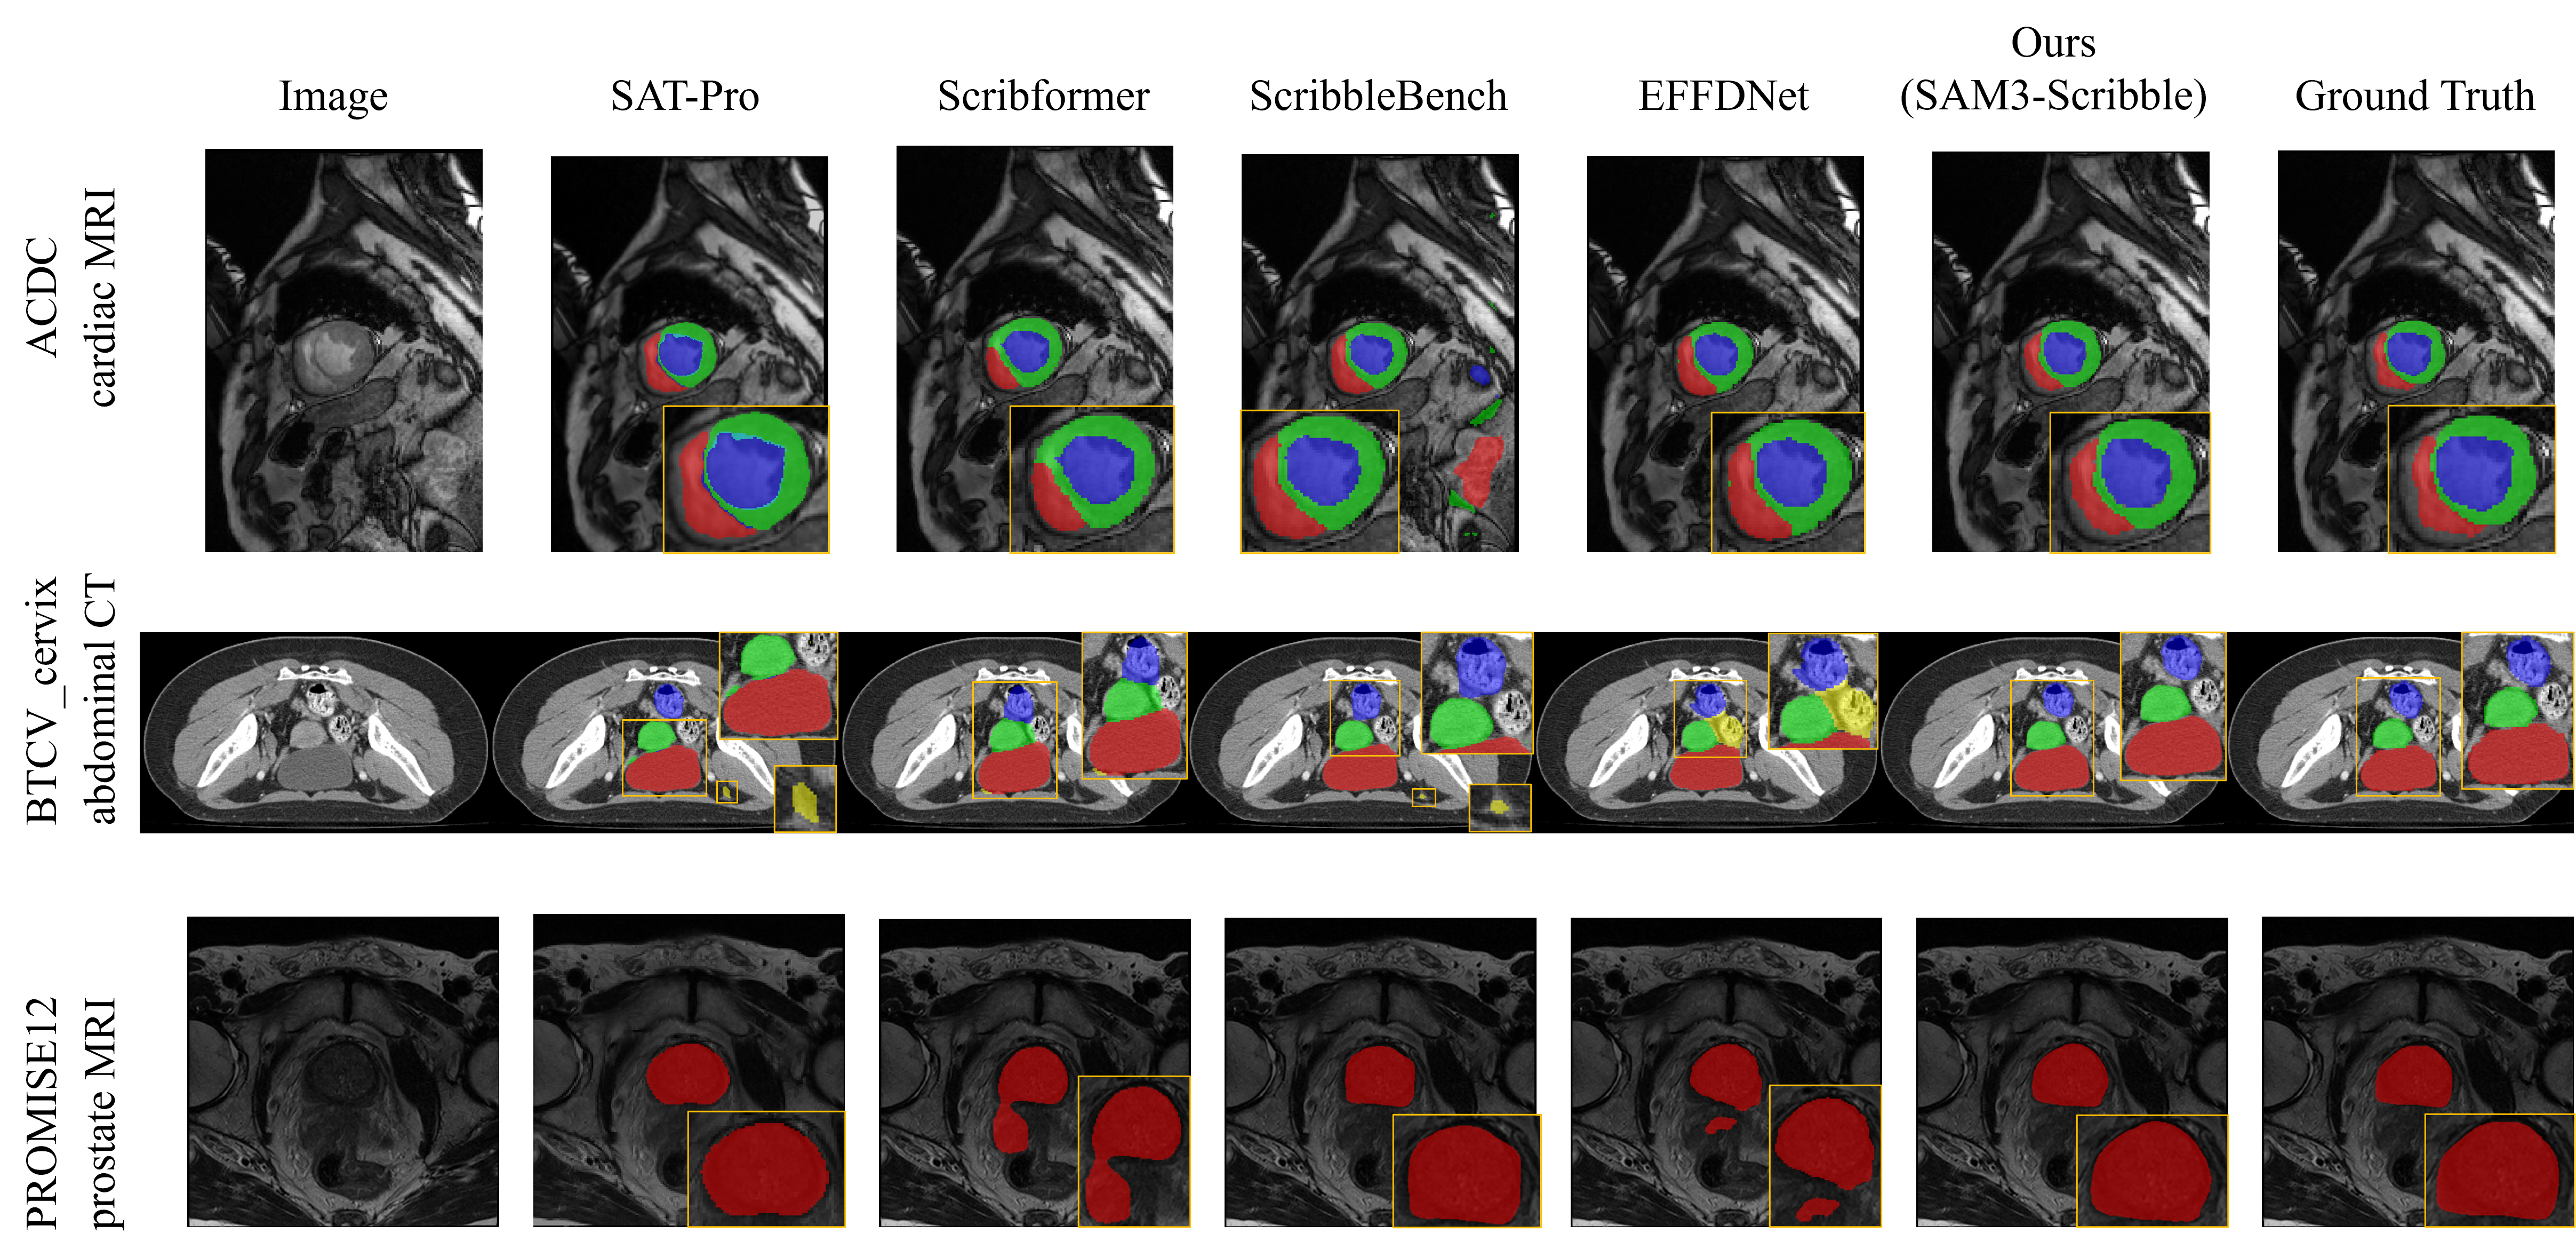
\includegraphics[width=\textwidth]{Figure4.png}
\caption{Qualitative comparison on ACDC, BTCV\_cervix, and PROMISE12. From left to right: input image, SAT-Pro, ScribFormer, ScribbleBench, EFFDNet, SAM3-Scribble, and ground truth. Zoomed regions are outlined in yellow.}
\label{fig:qualitative_comparison}
\end{figure}

Figure~\ref{fig:qualitative_comparison} provides qualitative comparisons across the three datasets. SAT-Pro can produce anatomically implausible false-positive regions, particularly on the BTCV\_cervix example, while static scribble-supervised baselines show case-dependent errors such as incomplete structures, irregular boundaries, or small spurious components. SAM3-Scribble yields masks that are more spatially coherent and closer to the ground truth in the highlighted regions, especially for the cardiac structures, pelvic organs, and prostate boundary. These observations are consistent with the quantitative trends in Tables~\ref{tab:main_results_acdc}--\ref{tab:main_results_promise12}; detailed per-structure results are provided in Supplementary Tables~S1--S3.

\FloatBarrier

\section{Discussion}
\label{sec:discussion}

The results demonstrate that a promptable segmentation foundation model can be adapted to medical image segmentation using sparse scribbles rather than dense masks. The key technical issue is not merely parameter-efficient fine-tuning, but the mismatch between scribble labels and the geometric assumptions of DETR-style training. The proposed partial mask loss directly addresses unlabeled pixels by excluding them from mask supervision, while removing box/GIoU regression and geometric matching costs reduces dependence on unreliable scribble-derived boxes.

The ablation studies also indicate that adaptation capacity should be distributed across the text-image segmentation pathway. Updating only the final mask and scoring heads is insufficient, and restricting LoRA to the DETR side substantially degrades performance. Vision-only adaptation is a competitive lightweight alternative, but the hybrid LoRA configuration provides stronger overall Dice and surface Dice. The rank and threshold sensitivity results further suggest that the final configuration is a stable operating point rather than a single over-tuned setting.

This study focuses on text-prompted segmentation rather than iterative point-, box-, or click-based interaction. This choice provides a zero-click workflow in which the anatomical category name is sufficient to request a segmentation, but it should not be interpreted as a full evaluation of all interactive modes supported by SAM3. Future work should compare text-only prompting with iterative spatial prompts and should quantify the value of scribble structure relative to equivalent sparse point supervision.

Another limitation is the slice-wise 2D formulation. Although this design makes direct use of the SAM3 image model and avoids assumptions about anisotropic volume spacing, it does not explicitly model inter-slice consistency. Future extensions could incorporate adjacent-slice context or tracking-based propagation to improve 3D coherence.

\section{Conclusion}

We presented a scribble-supervised adaptation of SAM3 for text-prompted medical image segmentation. By removing unreliable geometric regression losses and matching costs, and introducing a partial mask loss over explicitly labeled pixels, the proposed method enables SAM3 fine-tuning with sparse scribble annotations. Experiments on three medical datasets show that SAM3-Scribble approaches the performance of a fully supervised SAM3 model while substantially reducing annotation requirements. This provides a practical route for adapting promptable foundation models to medical segmentation tasks under limited annotation budgets.

\section*{CRediT authorship contribution statement}

Qi Gao: Conceptualization, Methodology, Software, Validation, Writing -- original draft. Huihui Fang: Methodology, Investigation, Supervision, Writing -- review and editing. Yanwu Xu: Supervision, Project administration, Writing -- review and editing.

\section*{Declaration of competing interest}

The authors declare that they have no known competing financial interests or personal relationships that could have appeared to influence the work reported in this paper.

\section*{Funding}

This research did not receive any specific grant from funding agencies in the public, commercial, or not-for-profit sectors.

\section*{Data and code availability}

The public datasets used in this study are available from their original providers. Code and trained model checkpoints will be made available upon publication.

\section*{Declaration of generative AI and AI-assisted technologies}

During preparation of this draft, AI-assisted tools were used to help convert the manuscript format and improve language. The authors reviewed and edited the content and take full responsibility for the final manuscript.

\begin{thebibliography}{10}
\expandafter\ifx\csname url\endcsname\relax
  \def\url#1{\texttt{#1}}\fi
\expandafter\ifx\csname urlprefix\endcsname\relax\def\urlprefix{URL }\fi
\expandafter\ifx\csname href\endcsname\relax
  \def\href#1#2{#2} \def\path#1{#1}\fi

\bibitem{ronneberger2015unet}
O.~Ronneberger, P.~Fischer, T.~Brox, {U-Net}: Convolutional networks for
  biomedical image segmentation, in: Medical Image Computing and
  Computer-Assisted Intervention -- MICCAI 2015, 2015, pp. 234--241.
\newblock \href {https://doi.org/10.1007/978-3-319-24574-4\_28}
  {\path{doi:10.1007/978-3-319-24574-4\_28}}.

\bibitem{isensee2021nnunet}
F.~Isensee, P.~F. Jaeger, S.~A.~A. Kohl, J.~Petersen, K.~H. Maier-Hein,
  {nnU-Net}: A self-configuring method for deep learning-based biomedical image
  segmentation, Nature Methods (2021).
\newblock \href {https://doi.org/10.1038/s41592-020-01008-z}
  {\path{doi:10.1038/s41592-020-01008-z}}.

\bibitem{kirillov2023sam}
A.~Kirillov, E.~Mintun, N.~Ravi, H.~Mao, C.~Rolland, L.~Gustafson, T.~Xiao,
  S.~Whitehead, A.~C. Berg, W.-Y. Lo, et~al., Segment anything, in: Proceedings
  of the IEEE/CVF international conference on computer vision, 2023, pp.
  4015--4026.

\bibitem{carion2025sam3}
N.~Carion, L.~Gustafson, Y.-T. Hu, S.~Debnath, R.~Hu, D.~Suris, C.~Ryali, K.~V.
  Alwala, H.~Khedr, A.~Huang, et~al., {SAM} 3: Segment anything with concepts,
  arXiv preprint arXiv:2511.16719 (2025).

\bibitem{zhao2025biomedparse}
T.~Zhao, Y.~Gu, J.~Yang, N.~Usuyama, H.~H. Lee, S.~Kiblawi, T.~Naumann, J.~Gao,
  A.~Crabtree, J.~Abel, C.~Moung-Wen, B.~Piening, C.~Bifulco, M.~Wei, H.~Poon,
  S.~Wang, A foundation model for joint segmentation, detection and recognition
  of biomedical objects across nine modalities, Nature Methods (2025).
\newblock \href {https://doi.org/10.1038/s41592-024-02499-w}
  {\path{doi:10.1038/s41592-024-02499-w}}.

\bibitem{zhao2025sat}
Z.~Zhao, Y.~Zhang, C.~Wu, X.~Zhang, X.~Zhou, Y.~Zhang, Y.~Wang, W.~Xie,
  Large-vocabulary segmentation for medical images with text prompts, npj
  Digital Medicine (2025).
\newblock \href {https://doi.org/10.1038/s41746-025-01964-w}
  {\path{doi:10.1038/s41746-025-01964-w}}.

\bibitem{rokuss2026voxtell}
M.~Rokuss, M.~Langenberg, Y.~Kirchhoff, F.~Isensee, B.~Hamm, C.~Ulrich,
  S.~Regnery, L.~Bauer, E.~Katsigiannopulos, T.~Norajitra, K.~Maier-Hein,
  {VoxTell}: Free-text promptable universal {3D} medical image segmentation,
  Accepted to the IEEE/CVF Conference on Computer Vision and Pattern
  Recognition (2026).
\newblock \href {https://doi.org/10.48550/arXiv.2511.11450}
  {\path{doi:10.48550/arXiv.2511.11450}}.

\bibitem{han2024DMSPS}
M.~Han, X.~Luo, X.~Xie, W.~Liao, S.~Zhang, T.~Song, G.~Wang, S.~Zhang, {DMSPS}:
  Dynamically mixed soft pseudo-label supervision for scribble-supervised
  medical image segmentation, Medical Image Analysis (2024).
\newblock \href {https://doi.org/10.1016/j.media.2024.103274}
  {\path{doi:10.1016/j.media.2024.103274}}.

\bibitem{li2024ScribFormer}
Z.~Li, Y.~Zheng, D.~Shan, S.~Yang, Q.~Li, B.~Wang, Y.~Zhang, Q.~Hong, D.~Shen,
  {ScribFormer}: Transformer makes {CNN} work better for scribble-based medical
  image segmentation, IEEE Transactions on Medical Imaging (2024).
\newblock \href {https://doi.org/10.1109/TMI.2024.3363190}
  {\path{doi:10.1109/TMI.2024.3363190}}.

\bibitem{liu2025effdnet}
J.~Liu, S.~Y. Tan, X.~Yang, Y.~Xu, S.~Y. Yeo, {EFFDNet}: A scribble-supervised
  medical image segmentation method with enhanced foreground feature
  discrimination, in: Medical Image Computing and Computer Assisted
  Intervention -- MICCAI 2025, Springer, 2025, pp. 194--204.

\bibitem{gotkowski2025scribblebench}
K.~Gotkowski, K.~H. Maier-Hein, F.~Isensee, Revisiting {3D} medical scribble
  supervision: Benchmarking beyond cardiac segmentation, arXiv preprint
  arXiv:2403.12834 (2025).

\bibitem{carion2020detr}
N.~Carion, F.~Massa, G.~Synnaeve, N.~Usunier, A.~Kirillov, S.~Zagoruyko,
  End-to-end object detection with transformers, in: Computer Vision -- ECCV
  2020, 2020, pp. 213--229.
\newblock \href {https://doi.org/10.1007/978-3-030-58452-8\_13}
  {\path{doi:10.1007/978-3-030-58452-8\_13}}.

\bibitem{hatamizadeh2022unetr}
A.~Hatamizadeh, Y.~Tang, V.~Nath, D.~Yang, A.~Myronenko, B.~Landman, H.~R.
  Roth, D.~Xu, {UNETR}: Transformers for {3D} medical image segmentation, in:
  Proceedings of the IEEE/CVF Winter Conference on Applications of Computer
  Vision, 2022, pp. 574--584.

\bibitem{rezatofighi2019giou}
H.~Rezatofighi, N.~Tsoi, J.~Gwak, A.~Sadeghian, I.~Reid, S.~Savarese,
  Generalized intersection over union: A metric and a loss for bounding box
  regression, in: Proceedings of the IEEE/CVF Conference on Computer Vision and
  Pattern Recognition, 2019, pp. 658--666.

\bibitem{hu2021lora}
E.~J. Hu, Y.~Shen, P.~Wallis, Z.~Allen-Zhu, Y.~Li, S.~Wang, L.~Wang, W.~Chen,
  {LoRA}: Low-rank adaptation of large language models, International
  Conference on Learning Representations (2022).

\bibitem{bernard2018acdc}
O.~Bernard, A.~Lalande, C.~Zotti, F.~Cervenansky, X.~Yang, P.-A. Heng,
  I.~Cetin, K.~Lekadir, O.~Camara, M.~A. Gonzalez~Ballester, G.~Sanroma,
  S.~Napel, S.~Petersen, G.~Tziritas, E.~Grinias, M.~Khened, V.~A. Kollerathu,
  G.~Krishnamurthi, M.-M. Roh{\\'e}, X.~Pennec, M.~Sermesant, F.~Isensee,
  P.~J{\\\"a}ger, K.~H. Maier-Hein, P.~M. Full, I.~Wolf, S.~Engelhardt, C.~F.
  Baumgartner, L.~M. Koch, J.~M. Wolterink, I.~I{\\v{s}}gum, Y.~Jang, Y.~Hong,
  J.~Patravali, S.~Jain, O.~Humbert, P.-M. Jodoin, Deep learning techniques for
  automatic {MRI} cardiac multi-structures segmentation and diagnosis: Is the
  problem solved?, IEEE Transactions on Medical Imaging (2018).
\newblock \href {https://doi.org/10.1109/TMI.2018.2837502}
  {\path{doi:10.1109/TMI.2018.2837502}}.

\bibitem{landman2015btcv}
B.~Landman, Z.~Xu, J.~Igelsias, M.~Styner, T.~Langerak, A.~Klein, {MICCAI}
  multi-atlas labeling beyond the cranial vault--workshop and challenge, in:
  Proc. MICCAI multi-atlas labeling beyond cranial vault--workshop challenge,
  Vol.~5, Munich, Germany, 2015, p.~12.

\bibitem{litjens2014promise}
G.~Litjens, R.~Toth, W.~Van De~Ven, C.~Hoeks, S.~Kerkstra, B.~Van~Ginneken,
  G.~Vincent, G.~Guillard, N.~Birbeck, J.~Zhang, R.~Strand, F.~Malmberg, Y.~Ou,
  C.~Davatzikos, M.~Kirschner, F.~Jung, J.~Yuan, W.~Qiu, Q.~Gao, P.~Edwards,
  B.~Maan, F.~Van Der~Heijden, S.~Ghose, J.~Mitra, J.~Dowling, D.~Barratt,
  H.~Huisman, A.~Madabhushi, Evaluation of prostate segmentation algorithms for
  {MRI}: The {PROMISE12} challenge, Medical Image Analysis (2014).
\newblock \href {https://doi.org/10.1016/j.media.2013.12.002}
  {\path{doi:10.1016/j.media.2013.12.002}}.

\bibitem{zhang2023samed}
K.~Zhang, D.~Liu, Customized {Segment} {Anything} {Model} for medical image
  segmentation, arXiv preprint arXiv:2304.13785 (2023).

\bibitem{wu2025medicalsamadapter}
J.~Wu, Z.~Wang, M.~Hong, W.~Ji, H.~Fu, Y.~Xu, M.~Xu, Y.~Jin, {Medical SAM
  Adapter}: Adapting {Segment Anything Model} for medical image segmentation,
  Medical Image Analysis 102 (2025) 103547.

\bibitem{cheng2023sammed2d}
J.~Cheng, J.~Ye, Z.~Deng, J.~Chen, T.~Li, H.~Wang, Y.~Su, Z.~Huang, J.~Chen,
  L.~Jiang, et~al., {SAM-Med2D}, arXiv preprint arXiv:2308.16184 (2023).

\bibitem{ma2024medsam}
J.~Ma, Y.~He, F.~Li, L.~Han, C.~You, B.~Wang, Segment anything in medical
  images, Nature Communications 15 (2024) 654.
\newblock \href {https://doi.org/10.1038/s41467-024-44824-z}
  {\path{doi:10.1038/s41467-024-44824-z}}.

\bibitem{gong2024threedsamadapter}
S.~Gong, Y.~Zhong, W.~Ma, J.~Li, Z.~Wang, J.~Zhang, P.-A. Heng, Q.~Dou,
  {3DSAM}-adapter: Holistic adaptation of {SAM} from {2D} to {3D} for
  promptable tumor segmentation, Medical Image Analysis 98 (2024) 103324.
\newblock \href {https://doi.org/10.1016/j.media.2024.103324}
  {\path{doi:10.1016/j.media.2024.103324}}.

\bibitem{chen2023masam}
C.~Chen, J.~Miao, D.~Wu, Z.~Yan, S.~Kim, J.~Hu, A.~Zhong, Z.~Liu, L.~Sun,
  X.~Li, T.~Liu, P.-A. Heng, Q.~Li, {MA-SAM}: Modality-agnostic {SAM}
  adaptation for {3D} medical image segmentation, arXiv preprint
  arXiv:2309.08842 (2023).
\newblock \href {https://doi.org/10.48550/arXiv.2309.08842}
  {\path{doi:10.48550/arXiv.2309.08842}}.

\bibitem{ma2025medsam2}
J.~Ma, Z.~Yang, S.~Kim, B.~Chen, M.~Baharoon, A.~Fallahpour, R.~Asakereh,
  H.~Lyu, B.~Wang, {MedSAM2}: Segment anything in {3D} medical images and
  videos, arXiv preprint arXiv:2504.03600 (2025).
\newblock \href {https://doi.org/10.48550/arXiv.2504.03600}
  {\path{doi:10.48550/arXiv.2504.03600}}.

\bibitem{lin2016ScribbleSup}
D.~Lin, J.~Dai, J.~Jia, K.~He, J.~Sun, {ScribbleSup}: Scribble-supervised
  convolutional networks for semantic segmentation, in: 2016 IEEE Conference on
  Computer Vision and Pattern Recognition (CVPR), 2016, pp. 3159--3167.
\newblock \href {https://doi.org/10.1109/CVPR.2016.344}
  {\path{doi:10.1109/CVPR.2016.344}}.

\bibitem{wang2018deepigeos}
G.~Wang, M.~A. Zuluaga, W.~Li, R.~Pratt, P.~A. Patel, M.~Aertsen, T.~Doel,
  A.~L. David, J.~Deprest, S.~Ourselin, et~al., {DeepIGeoS}: A deep interactive
  geodesic framework for medical image segmentation, IEEE Transactions on
  Pattern Analysis and Machine Intelligence 41~(7) (2018) 1559--1572.

\bibitem{zhang2022cyclemix}
K.~Zhang, X.~Zhuang, {CycleMix}: A holistic strategy for medical image
  segmentation from scribble supervision, in: Proceedings of the IEEE/CVF
  Conference on Computer Vision and Pattern Recognition, 2022, pp.
  11656--11665.

\bibitem{chen2025crossimage}
J.~Chen, W.~Huang, J.~Zhang, K.~Debattista, J.~Han, Addressing inconsistent
  labeling with cross image matching for scribble-based medical image
  segmentation, IEEE Transactions on Image Processing 34 (2025) 842--853.
\newblock \href {https://doi.org/10.1109/TIP.2025.3530787}
  {\path{doi:10.1109/TIP.2025.3530787}}.

\bibitem{zhang2025medcl}
K.~Zhang, V.~M. Patel, {MedCL}: Learning consistent anatomy distribution for
  scribble-supervised medical image segmentation, arXiv preprint
  arXiv:2503.22890 (2025).
\newblock \href {https://doi.org/10.48550/arXiv.2503.22890}
  {\path{doi:10.48550/arXiv.2503.22890}}.

\bibitem{zhang2024modelmix}
K.~Zhang, V.~M. Patel, {ModelMix}: A new model-mixup strategy to minimize
  vicinal risk across tasks for few-scribble based cardiac segmentation, in:
  Medical Image Computing and Computer Assisted Intervention -- MICCAI 2024,
  Springer, 2024, pp. 456--466.

\bibitem{boettcher2024scribblesforall}
W.~Boettcher, L.~Hoyer, O.~Unal, J.~E. Lenssen, B.~Schiele, Scribbles for all:
  Benchmarking scribble supervised segmentation across datasets, Advances in
  Neural Information Processing Systems 37 (2024).

\bibitem{zhang2026zscribbleseg}
K.~Zhang, B.~Wang, H.~Zhou, X.~Zhuang, {ZScribbleSeg}: A comprehensive
  segmentation framework with modeling of efficient annotation and maximization
  of scribble supervision, arXiv preprint arXiv:2605.06266 (2026).
\newblock \href {https://doi.org/10.48550/arXiv.2605.06266}
  {\path{doi:10.48550/arXiv.2605.06266}}.

\bibitem{kuhn1955hungarian}
H.~W. Kuhn, The {Hungarian} method for the assignment problem, Naval Research
  Logistics Quarterly 2~(1-2) (1955) 83--97.

\bibitem{Lin2017focal}
T.-Y. Lin, P.~Goyal, R.~Girshick, K.~He, P.~Dollar, Focal loss for dense object
  detection, in: Proceedings of the IEEE International Conference on Computer
  Vision (ICCV), 2017, pp. 2980--2988.

\bibitem{milletari2016dice}
F.~Milletari, N.~Navab, S.-A. Ahmadi, {V-Net}: Fully convolutional neural
  networks for volumetric medical image segmentation, in: 2016 Fourth
  International Conference on 3D Vision (3DV), 2016, pp. 565--571.
\newblock \href {https://doi.org/10.1109/3DV.2016.79}
  {\path{doi:10.1109/3DV.2016.79}}.

\bibitem{valvano2021scribbles}
G.~Valvano, A.~Leo, S.~A. Tsaftaris, Learning to segment from scribbles using
  multi-scale adversarial attention gates, IEEE Transactions on Medical Imaging
  40~(8) (2021) 1990--2001.
\newblock \href {https://doi.org/10.1109/TMI.2021.3059964}
  {\path{doi:10.1109/TMI.2021.3059964}}.

\bibitem{piegl2012nurbs}
L.~Piegl, W.~Tiller, The {NURBS} book, Springer Science \& Business Media,
  2012.

\bibitem{zhao2025boltzmann}
T.~Zhao, S.~Kiblawi, N.~Usuyama, H.~H. Lee, S.~Preston, H.~Poon, M.~Wei,
  Boltzmann attention sampling for image analysis with small objects, in:
  Proceedings of the IEEE/CVF Conference on Computer Vision and Pattern
  Recognition, 2025, pp. 25950--25959.

\end{thebibliography}


\end{document}
